\documentclass[11pt,english]{article}
\usepackage{geometry}
\usepackage{color}
\usepackage{graphicx}
\usepackage{float}
\usepackage{amsmath}

\makeatletter

%% User specified LaTeX commands.
\usepackage{color}
\usepackage[font=footnotesize,labelfont=bf]{caption}
\usepackage{listings}
\usepackage{pxfonts}
\usepackage{hyperref}
\usepackage{lmodern}
% To place footnotes at the bottom of the page
\usepackage[bottom]{footmisc}

% hyperref setup
\hypersetup{
  colorlinks=true,        % false: boxed links; true: colored links
  linkcolor=red,          % color of internal links (change box color with linkbordercolor)
  citecolor=green,        % color of links to bibliography
  filecolor=magenta,      % color of file links
  urlcolor=cyan           % color of external links
}

\geometry{verbose,a4paper,tmargin=3cm,bmargin=3cm,lmargin=2.5cm,rmargin=2.5cm,headheight=3cm,headsep=3cm}

\DeclareGraphicsExtensions{.png,.pdf,.jpg}

\setlength{\parskip}{\smallskipamount}
\setlength{\parindent}{0pt}
\renewcommand{\rmdefault}{cmr}
\renewcommand{\familydefault}{\rmdefault}

% Scientific notation
\providecommand{\e}[1]{\ensuremath{\times 10^{#1}}}

% Monospaced font with bold typeface
\DeclareFontShape{OT1}{cmtt}{bx}{n}{<5><6><7><8><9><10><10.95><12><14.4><17.28><20.74><24.88>cmttb10}{}

% Colors for listings
\definecolor{colKey}{rgb}{0,0,1}
\definecolor{colId}{rgb}{0,0,0}
\definecolor{colComments}{rgb}{0.247,0.498,0.254}
\definecolor{colEmph}{rgb}{0.498,0.286,0}
\definecolor{colString}{rgb}{0.05,0,0.8}
\definecolor{grigino}{rgb}{0.93,0.93,0.93}
\definecolor{gray}{rgb}{0.7,0.7,0.7}


% Listings captions gray box
\DeclareCaptionFont{white}{\color{white}}
\DeclareCaptionFormat{listing}{%
  \parbox{\textwidth}{\colorbox{gray}{\parbox{0.986\textwidth}{#1#2#3}}\vskip-4pt}}
\captionsetup[lstlisting]{format=listing,labelfont=white,textfont=white}

% Listing options set
\lstset{
  basicstyle=\scriptsize\ttfamily,
  float,
  showstringspaces=false,
  lineskip=-1pt,
  extendedchars=true,
  numbers=left,
  stepnumber=1,
  numberstyle=\tiny,
  numbersep=5pt,
  xleftmargin=2em,
  xrightmargin=2em,
  breaklines,
  language=C++,
  identifierstyle=\color{colId}, 
  keywordstyle=\color{colKey}, 
  stringstyle=\color{colString}, 
  commentstyle=\color{colComments},
  frame=lrb,
  rulecolor=\color{gray},
  framexleftmargin=15pt,
  framexrightmargin=15pt,
  morekeywords={uint16_t,uint32_t,byte,boolean}
}

% Listings custom keywords
\lstset{emph={%  
    _nDisplay, _displays, _value, _digits, _index, _name, _bitOrder, _groups%
    },emphstyle={\color{colEmph}}%
}%

\usepackage{babel}
\makeatother

%  Style for code names into text 
\newcommand{\code}[1]{\texttt{#1}}


\begin{document}

\begin{titlepage}
\begin{center} 

~\\[1.5cm] 
\textbf{{\Huge SCOREBOARD PROJECT}
~\\[0.7cm]}
\LARGE{Electronic board \\
with 7-segments displays\\
and Arduino
~\\[0.8cm]
version 1.0.2}
~\\[1.6cm]

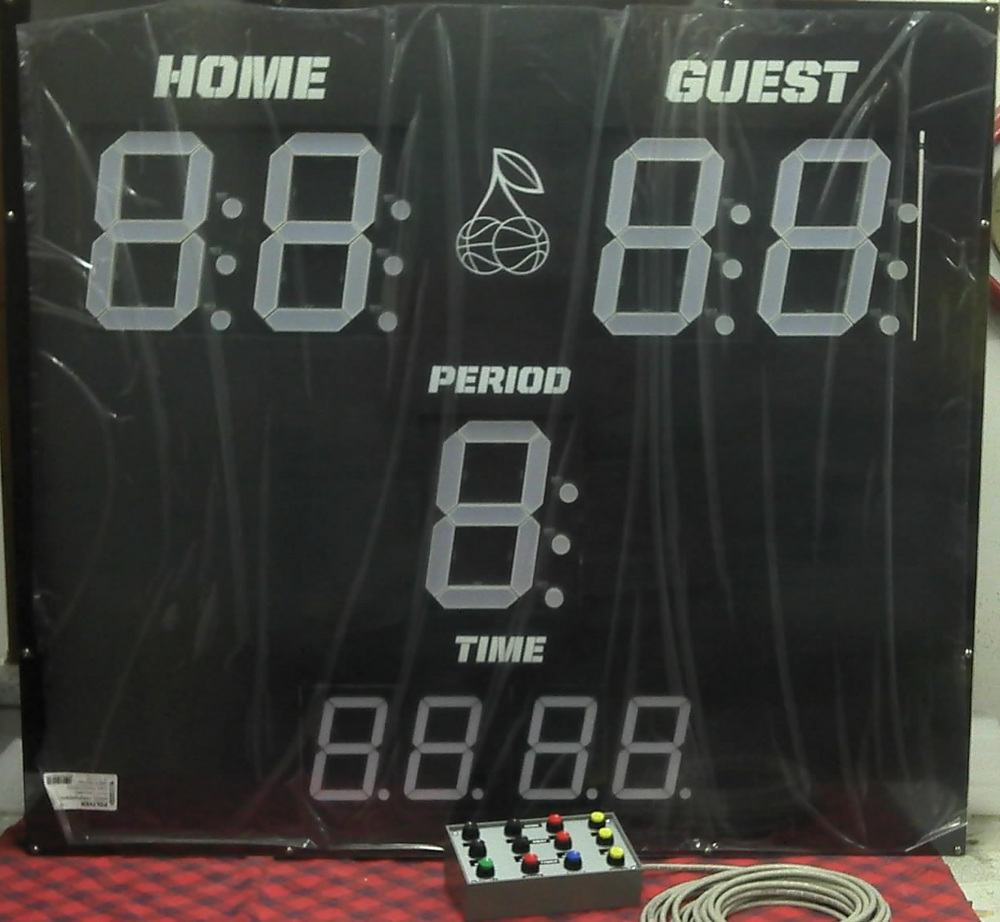
\includegraphics[scale=0.30]{img/Scoreboard}

~\\[1.5cm]
\normalsize Gionata Boccalini
~\\[0.5cm]
\normalsize \today

\end{center} 
\vspace*{1cm}
\end{titlepage}


\newpage{}

\tableofcontents{}


\listoffigures

\lstlistoflistings

\newpage{}



\section{Introduction}

This document describes the design and realization of an electronic scoreboard, 
that I was asked to make for my local basketball team. I had some experience with 
7-segments displays (from school) and with microelectronics so I decided to make 
my own scoreboard, using basic electronic blocks and Arduino as CPU. I had to seek 
for the right components on the Internet for months, and to put everything together 
in my garage, with the help of my father and some of my friends. Some parts were 
already made and some I had to build from scratch using tools that I would have never 
thought I used.The whole process took months but the final result was really 
impressive for me, given the knowledge and possibilities I had.

The rest of the document is organized in two main section, one describing the hardware 
part and the other speaking about the software. I will try to describe the most 
important aspects, using pictures, and give the main idea of simplicity and robustness 
that I tried to achieve.

I have to cite the source \footnote{\url{http://kiantech.me/entries/2011/6/21/live-nba-scoreboard.html}} 
where I found the inspiration to build this scoreboard, and from which I took some 
design hints. The site is run by Mr. Kianoosh Salami, who was really helping me in the 
process of finding the components and building the board.

I have also to thank many of my friends for the help, the knowledge the gave me and the
inspiration derived from the discovery of the \textquotedblleft Do it yourself\textquotedblright 
electronic field, represented by the Italian Arduino platform.   

Thank you!!

\section{Hardware}

The scoreboard has been completely realized by hand, starting from scratch, using wood 
for the chassis to create a box with an open side where I could put the electronic 
components. We made some holes for the 7-segments displays and the external connections.
Some pictures will explain better than words:

The chassis was robust enough to hold the displays, Arduino, and the wiring.
The list of components, with pictures, is shown in section \ref{subsec:components}.


\subsection{Components}\label{subsec:components}

The main components are:

\begin{itemize}
 \item 7-segments displays: I found those ones in a Chinese electronic company site, 
 Sure Electronics \footnote{\url{http://www.sureelectronics.net/goods.php?id=721}}, 
 selling worldwide, and I was very lucky because those displays already integrates the 
 electronic logic to  control the data flow from the CPU to the integrated shift registers. 
 Thus I saved the  effort to make my own circuit to drive the displays!!
 
  %
  \begin{figure}[H]
  \centering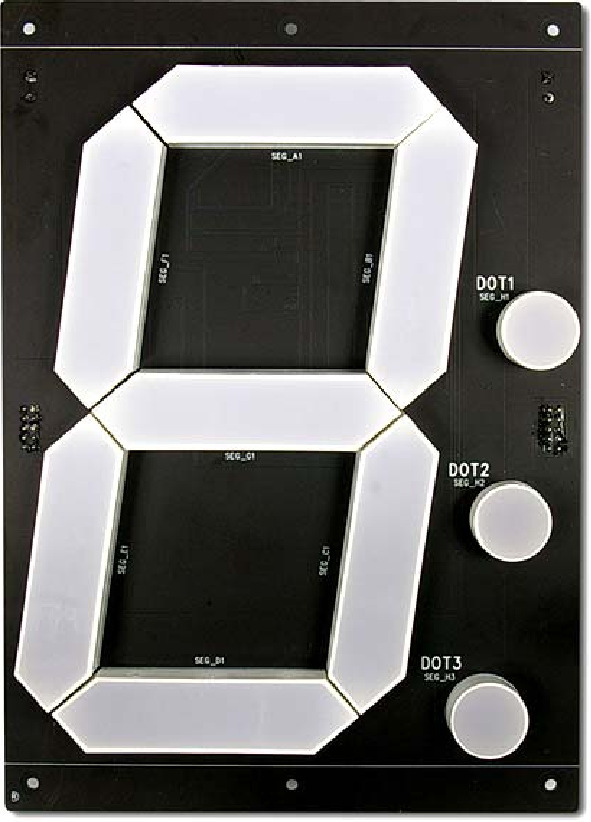
\includegraphics[scale=0.25]{img/7-inch-dis}

  \caption{A 7 inch 7-segments displays \label{fig:7-inch-dis}}

  \end{figure}
  
 \item Arduino: this is an Italian prototype platform really easy to use, with open source 
 software and standard hardware which helps non professional electronic designer and engineer 
 to develop their own application. I used this CPU to control the whole panel, the displays 
 and the digital inputs.
 
   %
  \begin{figure}[H]
  \centering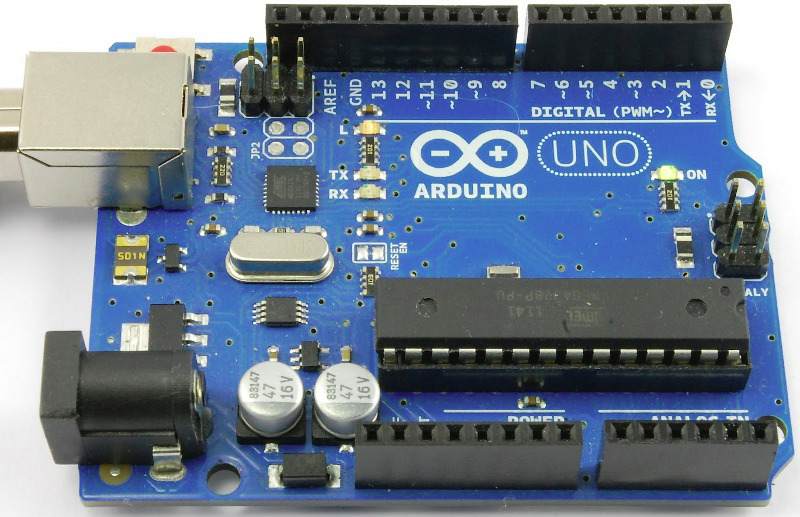
\includegraphics[scale=0.25]{img/Arduino}

  \caption{Arduino UNO platform\label{fig:arduino}}

  \end{figure}
 
 \item homemade connection boards: I used those ones to connect the CPU to the rest of the 
 circuit, like the control panel and the 7-segments displays. Later in this document or in the 
 download section of the project site \footnote{\url{http://code.google.com/p/display-group/}}  
 you can find the Eagle schematic and board files.
 
  %
  \begin{figure}[H]
  \centering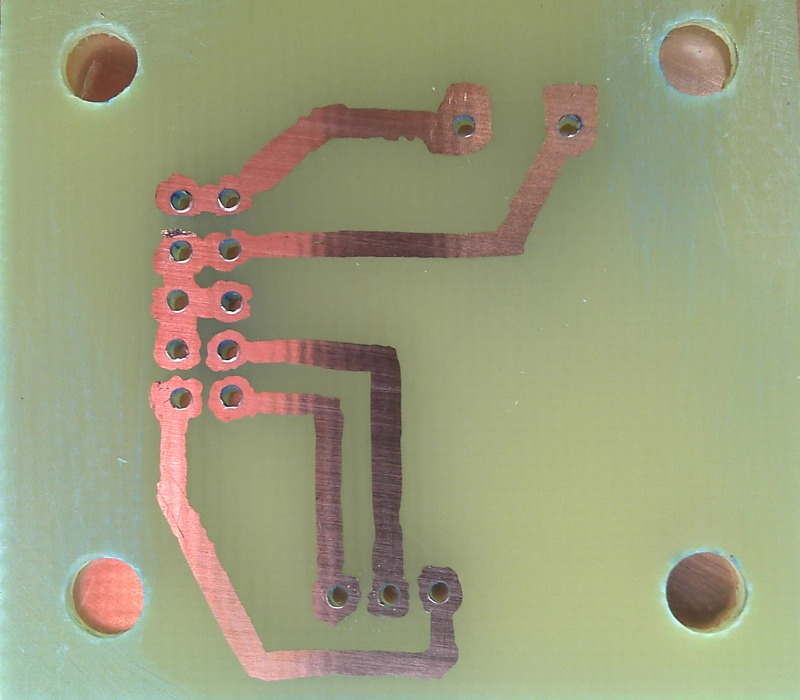
\includegraphics[scale=0.25]{img/Board}

  \caption{Homemade connection board without components \label{fig:board}}

  \end{figure}
 
 \item wood and DIY materials.
 
\end{itemize}


\subsection{ScoreBoard electrical connections}

The 7-segments are powered by a 12 V PSU, I decided to connect the power in parallel to all the boards:
the data link can carry 1 A current, but that is not enough to power 7 displays boards on the same bus.
Considering that Arduino is also powered by the same PSU, and the input are also, I used a 6.75 A, 12 V
PSU, just to be sure the current would be enough for everything.
The figure \ref{fig:board-back} shows the back of the scoreboard with all the components:

%
\begin{figure}[htb]
\centering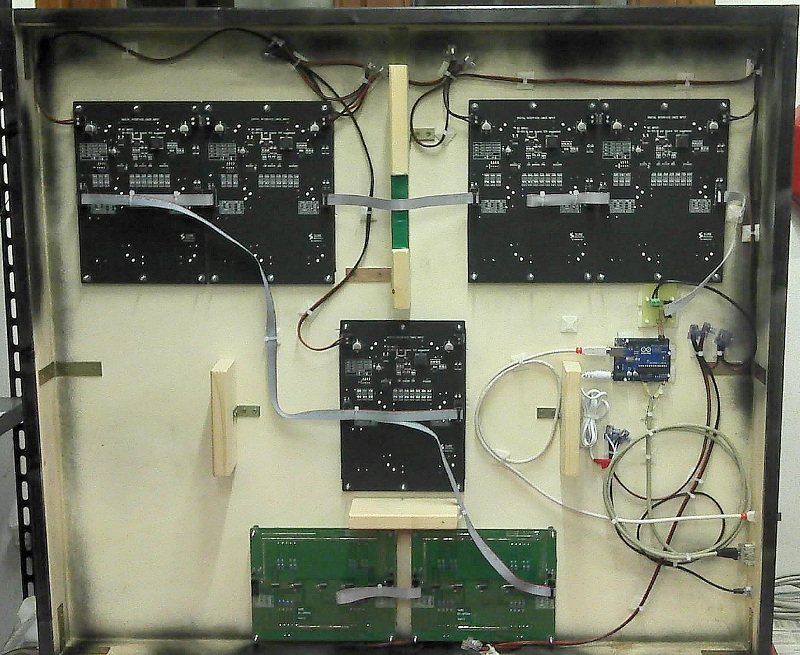
\includegraphics[scale=0.42]{img/Board-back}

\caption{Back side of the board, with Arduino and electrical connections \label{fig:board-back}}

\end{figure}

You can also see the external connections, in the bottom right corner:

\begin{itemize}
 \item Power cord: to power the whole board;
 \item USB: to program the Arduino when the board will be installed on the wall;
 \item Ethernet: to connect the control panel.
\end{itemize}

The data link between the CPU and the displays is made with a 10 pole IDC cable, with three data pins, 
as shown in figure \ref{fig:j1}. 

%
\begin{figure}[htb]
\centering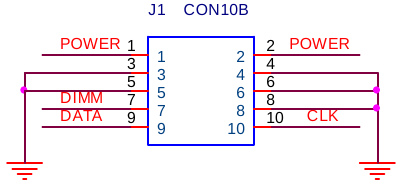
\includegraphics[scale=0.45]{img/J1-con}

\caption{Power and data connection on the 7-segments board \label{fig:j1}}

\end{figure}

The pins are described as follows
\begin{itemize}
 \item \textbf{DIMM/OE}: to control the brightness of the LEDs and the output enable of the shift registers;
 \item \textbf{DATA}: to shift in data bits;
 \item \textbf{CLK}: to clock the data bits on the bus.
\end{itemize}

To have more information on the displays and the electronic behind look on the project site, download 
section, for the displays datasheets.

I used an electronic board to make the data connection persistent, as shown in figure \ref{fig:board}, 
with standard connectors soldered on it: figure \ref{fig:board-schem} shows the board PCB circuit made with 
Eagle CAD software.

%
\begin{figure}[htb]
\centering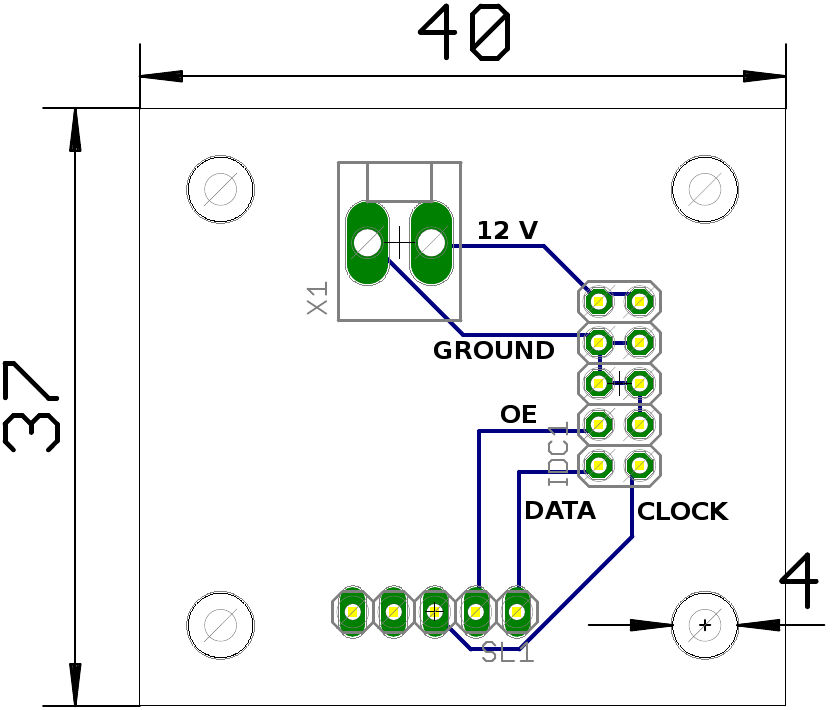
\includegraphics[scale=0.30]{img/Board-schem}

\caption{Connection board schematic \label{fig:board-schem}}

\end{figure}

The OE, DATA, CLOCK pins come from Arduino, and are routed to the IDC connector, together with the 12 V line and 
ground. The IDC cable goes to the first 7-segments display (top right corner in figure \ref{fig:board-back})
the IDC output connector goes to the second display on its left, and so on. Using a digital shift out technique 
on Arduino it is possible to update all the displays at a time. The DisplayGroup library has been used for this 
purpose.

The two displays at the bottom of figure \ref{fig:board-back} are the last two of the queue: they are 4 inch tall 
and use the same hardware interface of the 7 inch displays, but the segments bit code is different!
The DisplayGroup library can handle this representation difference in transparent way to the user.


\subsection{Control panel}\label{subsec:contro-panel}

The small control panel shown in figure \ref{fig:panel} has been built to give the user the possibility 
to remotely control the scoreboard during the game. The buttons are described in picture \ref{fig:panel-schem}.

%
\begin{figure}[htb]
\centering\includegraphics[scale=0.35]{img/Panel}

\caption{Control panel \label{fig:panel}}

\end{figure}

There is a \textquotedblleft shift\textquotedblright like button to enable additional function like the set 
of the timer and the reset of score.

%
\begin{figure}[H]
\centering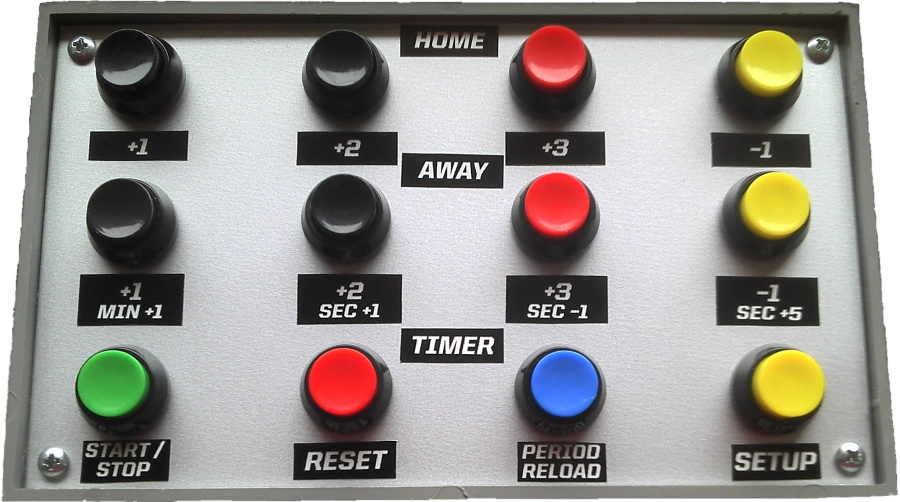
\includegraphics[scale=0.35]{img/Panel-schem}

\caption{Control panel front view \label{fig:panel-schem}}

\end{figure}

The panel is powered by the Arduino 5 V output through the Ethernet cable; this is the only cable needed to make 
the panel work: it brings the power and the data link, using only five cable out of the eight present in the 
Ethernet cable.
Those cables are mapped to the Arduino analog input: this means that, since the buttons are digital switch, I 
had to build a board to extend the Arduino input capability: using only 3 analog input Arduino can receive 
12 digital inputs, with the correct resistors and the help of the software 
\footnote{\url{http://www.instructables.com/id/How-to-access-5-buttons-through-1-Arduino-input/?ALLSTEPS}}. 
The board schematic is shown in figure \ref{fig:panel-board}:

%
\begin{figure}[htb]
\centering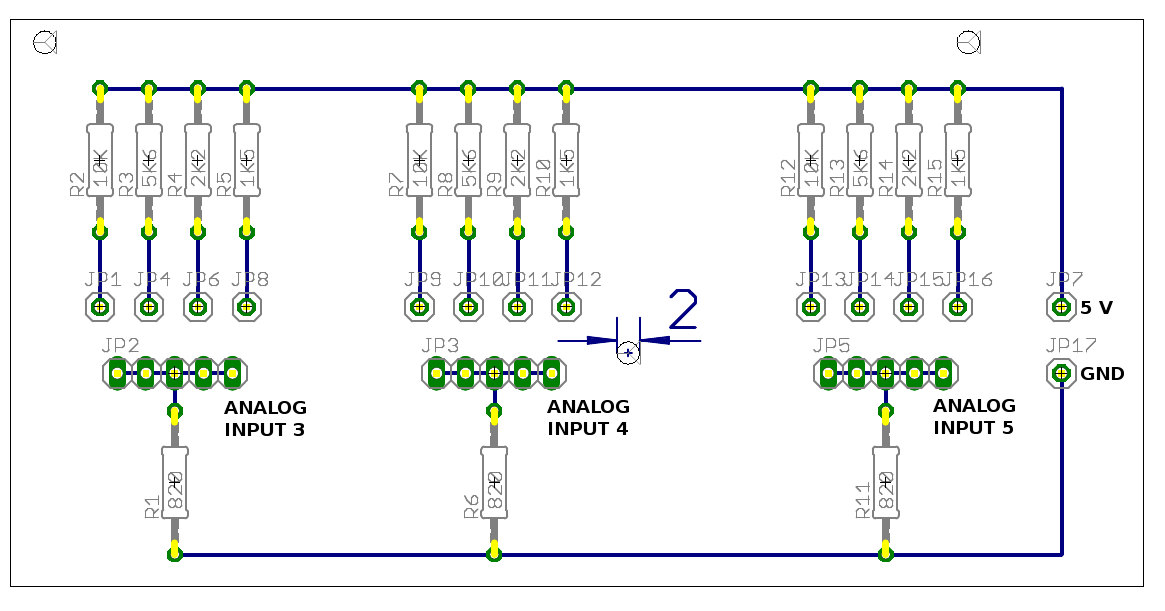
\includegraphics[scale=0.25]{img/Panel-board}

\caption{Control panel connection board \label{fig:panel-board}}

\end{figure}

The board is essentially a voltage divider with three voltage sample, one for each analog input: every button 
has its particular size of the divider resistor, so when the user pushes a button the corresponding voltage 
value goes to the correct analog input. Those values are hard coded into the control program on the CPU; 
the library for the input control scans the analogs input and calls the correct function when needed. This
library will be described in section \ref{subsec:dep}.

I used a straight Ethernet cable but, due to the necessary joints, I had to map the cable differently between the 
two communication sides: as you can see from picture \ref{fig:panel-cable} the orange-white e green-white 
cables are swapped:

%
\begin{figure}[htb]
\centering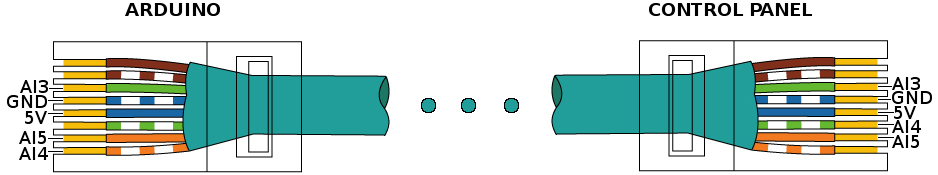
\includegraphics[scale=0.40]{img/Panel-cable}

\caption{Control panel connection board \label{fig:panel-cable}}

\end{figure}

By using this cabled solution I was able to control the scoreboard with a quite long cable (12 meters), 
while keeping the realization cost low. The other solution would be a wireless communication, but that 
would also be more expensive.

\pagebreak

\section{Software}

The control software is made of three library and a main logic, written in C++, with the use of Arduino 
API and C++ STL library (Arduino version). The README and INSTALL document in the root folder of the 
project explain where to find those libraries, and then you can understand how to compile them. The 
rest of the compilation process is done by Eclipse or by the makefile. Also the flashing of the program 
on the Arduino program memory is automatically done, provided that all the needed tools are installed.

\subsection{Dependences}\label{subsec:dep}

The most important dependence is the DisplayGroup library, which has already been described in the 
documentation at the project folder, on the Google code svn server (INSTALL file). This library is needed 
to support in an efficient way many 7-segments connected to a serial bus, each with a shift register, 
just like the situation in this project as shown in figure \ref{fig:board-back}.
The display configuration in this case is:

%
\begin{lstlisting}[label=lis:dis-config,caption=DisplayGroup configuration]
DisplayGroup::DisplayManager disManager(PIN_COM_DATA, PIN_COM_CLOCK, PIN_OUTPUT_ENABLE);

disManager.addGroup("Home_score", 2, 0, &score.home, gDigits7, sizeof(gDigits7));
disManager.addGroup("Away_score", 2, 1, &score.away, gDigits7, sizeof(gDigits7));
disManager.addGroup("Period", 1, 2, &time.period, gDigits7, sizeof(gDigits7));
disManager.addGroup("Timer_minutes", 2, 3, &time.min, gDigits4, sizeof(gDigits4));
disManager.addGroup("Timer_seconds", 2, 4, &time.sec, gDigits4, sizeof(gDigits4));
\end{lstlisting}

where \code{score} and \code{time} are struct I used to keep information regarding the match score and the 
actual time. \code{gDigits7} and \code{gDigit4} are arrays of segments code, necessary for the library 
configuration, respectively for 7 inches and 4 inches displays. 

The second dependence library is AnalogButtons \footnote{\url{http://playground.arduino.cc/Code/AnalogButtons}},
used to control many digital inputs through few analog inputs from the Arduino interface. The configuration 
for this library is:
%
\begin{lstlisting}[label=lis:buttons-config,caption=AnalogButtons configuration]
// Patch cable
const uint16_t bAVal[10] = { 60, 90, 120, 150, 250, 295, 340, 375 };


AnalogButtons homeButtons(HOME_ANALOG_INPUT, DEBOUNCING_COUNT_HOME, &handleHomeButtons);
Button b1 = Button(HOME_P1, bAVal[0], bAVal[1]);
Button b2 = Button(HOME_P2, bAVal[2], bAVal[3]);
Button b3 = Button(HOME_P3, bAVal[4], bAVal[5]);
Button b4 = Button(HOME_M1, bAVal[6], bAVal[7]);

AnalogButtons awayButtons(AWAY_ANALOG_INPUT, DEBOUNCING_COUNT, &handleAwayButtons);
Button b5 = Button(AWAY_P1, bAVal[0], bAVal[1]);
Button b6 = Button(AWAY_P2, bAVal[2], bAVal[3]);
Button b7 = Button(AWAY_P3, bAVal[4], bAVal[5]);
Button b8 = Button(AWAY_M1, bAVal[6], bAVal[7]);

AnalogButtons timerButtons(TIMER_ANALOG_INPUT, DEBOUNCING_COUNT, &handleTimerButtons);
Button b9 = Button(TIMER_START_STOP, bAVal[0], bAVal[1]);
Button b10 = Button(TIMER_RESET, bAVal[2], bAVal[3], HELD_DURATION);
Button b11 = Button(PERIOD_P1, bAVal[4], bAVal[5]);
Button b12 = Button(SETUP_MODE, bAVal[6], bAVal[7], HELD_DURATION);

...

// Input Buttons
homeButtons.addButton(b2);
homeButtons.addButton(b1);
homeButtons.addButton(b3);
homeButtons.addButton(b4);

awayButtons.addButton(b5);
awayButtons.addButton(b6);
awayButtons.addButton(b7);
awayButtons.addButton(b8);

timerButtons.addButton(b9);
timerButtons.addButton(b10);
timerButtons.addButton(b11);
timerButtons.addButton(b12);

\end{lstlisting}

I used three analog inputs to control twelve digital inputs, called buttons in the program. 
For each analog input there is a callback function: \code{handleHomeButtons}, \code{handleAwayButtons}  
and \code{handleTimerButtons}. In these functions is implemented the control logic for each buttons.
Some of the buttons have an \code{HELD\_DURATION} options: these inputs must be held for some seconds to
become active.


\subsection{Main control program}

The main program is composed by the three library described in section \ref{subsec:dep} and by a main 
program that will be described in this section. The structure of the main program is shown in \ref{lis:main-structure} 
there are three callbacks to handle the analog input, one to handle the timer interrupt, and some 
functions to manage the EEPROM memory.

%
\begin{lstlisting}[label=lis:main-structure,caption=Main program structure]

void handleHomeButtons(int id, boolean held) {}

void handleAwayButtons(int id, boolean held) {}

void handleTimerButtons(int id, boolean held) {}

void handleTime() {}

// #########################################################
// ####### EEPROM wear leveling algorithm functions ########
// #########################################################

void resetEEPROM() {}

boolean initializeEEPROM() {}

boolean writeEEPROM() {}

void printEEPROM() {}

// ========================================================
// |                        SETUP                         |
// ========================================================

void setup() {} 

// ========================================================
// |                        LOOP                          |
// ========================================================

void loop() {}
\end{lstlisting}

The \code{setup()} and \code{loop()} functions are necessary to the Arduino AVR compiler: 

\begin{itemize}
\item \code{setup()} provides the program initialization: it is used to configure the libraries
      and to check the state of the EEPROM memory (see \ref{subsubsec:wear-level});

\item \code{loop()} provides the main control loop: in this function the update of the displays is 
      executed and the actual state of the analog inputs is checked (see \ref{subsubsec:input-enable}).
\end{itemize}

The rest of the main program (the \code{main()} function) is automatically added by the Arduino library, 
so the final main program will be:

%
\begin{lstlisting}[label=lis:main-loop,caption=Main program from Arduino library]

#include <Arduino.h>

int main(void)
{
    init();

#if defined(USBCON)
    USBDevice.attach();
#endif
    
    setup();
    
    for (;;) {
        loop();
        if (serialEventRun) serialEventRun();
    }
        
    return 0;
}
\end{lstlisting}


\subsubsection{Input enable} \label{subsubsec:input-enable}

The digital inputs are mapped to the Arduino analog inputs through the board described in section 
\ref{subsec:contro-panel}. On the board the input are kept low with a pull down resistor. This means 
that when the input cable is disconnected the analog inputs are not connected to anything and they 
are not kept low! Thus the integer value read by Arduino is a random value between 0 and 1023.
This result in some weird behavior of the scoreboard like self-increasing score and timer disturbance 
because of the fake input. 

To fix this issue I had to realize a software check that, with some limitation, control the actual values 
of the analog inputs and disable the input when all three analog values are different than zero. This 
situation is met only when the cable is disconnected or when the user pushes at least one button on each 
row on the control panel (each row is connected to an analog input). The latter is again a dangerous 
situation so the input are going to be disable in both cases.
When all the three analog value are equal to zero the analog inputs are re-enabled, because this means that 
cable has been reconnected and the pull down resistors are working correctly.
The control sequence is implemented in the \code{loop()} function and is shown in listing \ref{lis:main-input}:
%
\begin{lstlisting}[label=lis:main-input,caption=Main program from Arduino library]

// Analog input not connected
if (!inputEnable) {
  int homeAnalogValue = analogRead(HOME_ANALOG_INPUT);
  // Delay before the next analogRead, for the analog-to-digital converter
  // to settle after the last reading
  delay(10);
  int awayAnalogValue = analogRead(AWAY_ANALOG_INPUT);
  delay(10);
  int timerAnalogValue = analogRead(TIMER_ANALOG_INPUT);
  delay(4);

  // This check works only if the analog input are kept low with a pull down
  // resistor!
  if (homeAnalogValue == 0 && awayAnalogValue == 0 && timerAnalogValue == 0) {
    inputEnable = true;
  }
} else {
  // Analog input connected, check for buttons pressed
  homeButtons.checkButtons();
  awayButtons.checkButtons();
  timerButtons.checkButtons();

  int homeAnalogValue = homeButtons.analogValue();
  int awayAnalogValue = awayButtons.analogValue();
  int timerAnalogValue = timerButtons.analogValue();

  // The analog inputs have been disconnected: "random" value will be on
  // each analog port (usually much greater than 0)
  if (homeAnalogValue != 0 && awayAnalogValue != 0 && timerAnalogValue != 0) {
    inputEnable = false;
  }
}
\end{lstlisting}

At the initialization the input are disabled and after they are constantly checked by using the Arduino 
API and the AnalogButtons library.
There is still a problems with this type of digital-to-analog inputs: when the user pushes two buttons 
of different row some weird behavior can happen, but after some tests of the scoreboard for many matches I 
can say this is not a real problem. Anyway this is not fixable with a software approach, instead a careful
choice of the resistors values is necessary to avoid such problems. 



\subsubsection{Countdown timer} \label{subsubsec:timer}


A basketball game, just like many other sports, requires a countdown timer to keep trace of the effective 
time in the game. This timer could be easily made using the \code{delay()} or \code{millis()} functions 
in the Arduino APIs, but since the precision matters I decided to use an hardware interrupt with precise 
calculation behind. 
The Arduino platform can generate some hardware interrupt using counters and the configuration is easy if 
you have some introduction to interrupt logic and setup in the microcontrollers field. If not you can read 
this good introduction \footnote{\url{http://www.engblaze.com/microcontroller-tutorial-avr-and-arduino-timer-interrupts/}},
which end up with exactly with the configuration I used. The Atmel AVR CPU datasheet is the resource where 
you can find some more detailed information on the internals configurations (for the Arduino Uno the 
CPU is the ATmega328p \footnote{\url{http://www.atmel.com/devices/ATMEGA328P.aspx}}).   

I will describe here only the configuration I used, since all the other information can be easily found at the 
resource I pointed to or elsewhere in the Internet.
I used the Clear Timer on Compare Match, or \emph{CTC}, interrupt on timer 1, with system clock as counter clock.
The timer compares its count to a value that was previously stored in a register. When the count matches that 
value, the timer can either set a flag or trigger an interrupt. The interrupt will be served by an \emph{ISR} 
(Interrupt Service Routine), in which the user can put the needed code.
Using a prescaler of 1024 the compare match value $T_c$ to fire the interrupt every second is 15624, considering 
the CPU frequency (16MHz). This value is obtained as

\[
 T_c = \left(  \frac{T_t}{T_r} \right) - 1 
\]

where $T_t$ is the timer target time, 1 s in this application, and $T_r$ is the time resolution given the CPU 
clock frequency and the prescaler, obtained as

\[
 T_r = \frac{prescaler}{CPU_f} = 6.4\e{-5} \, s
\]
 
Once the timer 1 reaches this value the ISR will be executed: 

%
\begin{lstlisting}[label=lis:timer-ISR,caption=Interrupt Service Routine]
ISR(TIMER1_COMPA_vect) {
  sec--;
  updateDisplay = true;
  saveEEprom = true;
}
\end{lstlisting}

The function manages the total seconds counter, and sets some flags to write the new time on the 
internal EEPROM and to refresh the displays. Thus, when the time is updated the new time is shown on the 
displays as soon as possible. 
Some care must be taken to avoid problems at runtime due to the compiler optimizations: the variables shared 
between the ISR and the rest of the code have to be declared \code{volatile}, and they have to be copied to 
a local variable in a interrupt free context, saving and restoring the status register (\emph{SREG}): 

%
\begin{lstlisting}[label=lis:main-timer,caption=Read shared variables in the main program ]
// Interrupt free context to update shared volatile variables
sreg = SREG;
cli();
updateDisplayLocal = updateDisplay;
saveEEpromLocal = saveEEprom;
updateDisplay = false;
saveEEprom = false;
secLocal = sec;
sei();
SREG = sreg;
\end{lstlisting}

The same special code should be used when setting and resetting the timer 1 counter value or the configuration 
registry, as shown in listings \ref{lis:setup-timer} and \ref{lis:timer-use}.

%
\begin{lstlisting}[label=lis:setup-timer,caption=Setup of the timer interrupt]
void setup() {
  ...
  // Setup of timer1 CTC interrupt
  // Initialize Timer1
  cli();          // disable global interrupts
  TCCR1A = 0;     // set entire TCCR1A register to 0
  TCCR1B = 0;     // same for TCCR1B

  // Set compare match register to desired timer count
  OCR1A = 15624;
  // Turn on CTC mode
  // TCCR1B |= (1 << WGM12);
  // Set CS10 and CS12 bits for 1024 prescaler
  // TCCR1B |= (1 << CS10);
  // TCCR1B |= (1 << CS12);
  // So its TCCR1B = 13 the make the timer start

  // Enable timer compare interrupt:
  TIMSK1 |= (1 << OCIE1A);
  sei();          // Enable global interrupts:
}
\end{lstlisting}


%
\begin{lstlisting}[label=lis:timer-use,caption=Use of the timer]
case TIMER_START_STOP:
      if (timerRunning) {
        // Stop timer, save global interrupt flag and restore after
        sreg = SREG;
        cli();
        TCCR1B = 0;
        SREG = sreg;

        timerRunning = false;
        updateDisplay = true;
      } else {
        // Start/restart timer
        if (time.min == 0 && time.sec == 0) {
          return;
        }
        sreg = SREG;
        cli();
        TCCR1B = 13;
        SREG = sreg;

        timerRunning = true;
        updateDisplay = true;
      }
      break;

    case TIMER_RESET:
      if (!timerRunning && held) {
        sreg = SREG;
        cli();
        TCNT1 = 0;
        SREG = sreg;

        time.min = TIMER_INIT_MIN;
        time.sec = TIMER_INIT_SEC;
        sec = TIMER_INIT_MIN * 60 + TIMER_INIT_SEC;
      }
      updateDisplay = true;
      break;
\end{lstlisting}


The accuracy in time of this interrupt depends on the stability of the crystal oscillator integrated in the CPU, 
which is +/- 50 ppm, so it is +/- 2 minutes clock's error during one month. If the crystal is working at constant 
room temperature stability should be even better.  



\subsubsection{EEPROM wear leveling} \label{subsubsec:wear-level}

The Arduino internal EEPROM memory has uniques electrically erasable cells, up to 1024 bytes. Each of these 
cell can be erases a limited number of time (erase cycle) before becoming unreliable. For the Arduino UNO r3
CPU the life is about 100000 erase cycle for \emph{each} cell. Since the erase cycle is executed 
also upon a write cycle the cell write cycles are limited too. A wear leveling algorithm attempts to work around 
these limitations by arranging data in a such a way that re-writes are distributed evenly across the medium. 
In this way no single erase cell prematurely fails due to a high concentration of write cycles. 

In this application the EEPROM memory is used to store the march data (score and time) and to restore them in 
case of power loss. I wanted to save every change in the data, so the time changes every second and this result 
in a write cycle for some cells in the memory. Also when the score changes it is written to the memory. 
Given that every basketball game is composed by at least 4 period, and each period lasts 10 minutes (effective 
time), the average number of writing command no the EEPROM per game is:

\[
W_m \simeq 60 \; seconds * 10 \; minutes * 4 \; periods + 100 \; score \, change \simeq 2500 writings
\]

I considered 100 additional writing to account for the score changes, which themselves generate an independent 
write cycle on the EEPROM.  

Each write cycle involves the whole amount of data shown in listing \ref{lis:persistent-data}:

%
\begin{lstlisting}[label=lis:persistent-data,caption=Persistent data type]
// ####################### Data types #######################
struct Score {
  uint16_t home;        // 2 bytes
  uint16_t away;        // 2 bytes
};

struct Time {
  uint16_t min;         // 2 bytes
  uint16_t sec;         // 2 bytes
  uint16_t period;      // 2 bytes
};

// Pesistend data type to be written on the EEPROM
struct persistentData {
  uint32_t counter;     // 4 bytes
  Score score;          // 4 bytes
  Time time;            // 6 bytes
};
\end{lstlisting}

The data type \code{persistentData} size is 14 bytes: so 14 cells will be written on each write command. The 
\code{counter} variable is used to keep trace of the how many writes have been executed on the cell group. If 
I used only one group of 14 cells the total memory life would be:

\[
L = \frac{100000}{W_m} = 40 \; games
\] 

This means that after only 40 games the first 14 cells of the EEPROM would have been written 100000 times, and thus 
the cells would be not reliable any more. But the EEPROM is made of 1024 cells that can be used! 

In my simple algorithm I decided to use $G = \lfloor\tfrac{1024}{14}\rfloor = 73$ groups, in this way I can use 
the whole memory, starting from the first group and shifting the write cycle on to the next group when the previous 
one has become unreliable, after 100000 write cycles. 
This procedure allows the application to last much longer, in particular:

\[
L = 73 \; * \; \frac{100000}{W_m} = 2920 \; games
\]

This life is more than enough for my need so, although the algorithm can be easily improved, I used this version of 
the wear leveling algorithm, implemented by some functions in the main program.

Those function use the \code{avr/eeprom.h} library found in the Arduino include directory to read and write the EEPROM 
cells. are:

\begin{description}
\item[\code{initializeEEPROM()}]:

Used to initialize the algorithm to write the EEPROM starting from the first not 
out of order cell, i.e. its life is not over. This function scans the whole memory and find the first usable cell,
than the rest of the algorithm will write starting from this location. If the memory is full, i.e. there are no 
remaining cells, the application will not save anything and the related functions will be not used.
This functions read also the last saved values if present, which can be restored at any time using the control 
panel in setup mode. The values are stored in RAM so that the application can still save the data when needed 
without overwrite the restore data in the EEPROM.
\end{description}

%
\begin{lstlisting}[label=lis:initializeEEPROM,caption=initializeEEPROM() function]
boolean initializeEEPROM() {
  persistentData data;

  uint16_t size = sizeof(data);

  uint16_t readCounter = (uint16_t) EEPROM_SIZE / size;

  for (uint16_t i = 0; i < readCounter; i++) {
    eeprom_read_block((void*) &data, (void*) (size * i), sizeof(data));

    if (data.counter < EEPROM_MAX_WRITE) {
      if (data.counter == 0 && i > 0) {
        // Read from previous cell, just reached end of life
        i--;
        eeprom_read_block((void*) &data, (void*) (size * i), sizeof(data));
      }
      counterEE = data.counter;
      offsetEE = size * i;
      dataEE = data;
      return true;
    }
  }

  // EEPROM full (end of life), read last saved data
  dataEE = data;
  return false;
}
\end{lstlisting}


\begin{description}
\item[\code{writeEEPROM()}]: 

Used to write the actual data to the EEPROM when requested by the application. The function writes the data and 
increment the actual write counter in the cell group. If the is no cells available the function simply returns.
\end{description}

%
\begin{lstlisting}[label=lis:writeEEPROM,caption=writeEEPROM() function]
boolean writeEEPROM() {
  persistentData data;
  uint16_t size = sizeof(data);

  counterEE++;

  if (counterEE > EEPROM_MAX_WRITE) {
    offsetEE += size;
    counterEE = 1;
  }

  if (offsetEE >= EEPROM_SIZE) {
    return false;
  }

  data.counter = counterEE;
  data.score = score;
  data.time = time;

  eeprom_write_block((void*) &data, (void*) offsetEE, sizeof(data));

  return true;
}
\end{lstlisting}

The are two other service functions: \code{readEEPROM()} and \code{printEEPROM()}: the former reads the data in the 
EEPROM at a specified offset, and the latter prints the EEPROM content to the serial interface, to show the actual 
state of the memory, for debug purpose.


\subsection{Volleyball mode}

In a recent release (v1.0.2) the volleyball mode has been implemented. This was done on requested from a volleyball 
coach, so I tried to adapt the software without touching the hardware (the scoreboard is already mounted on the wall 
by now). The new mode simply changes the meaning of some displays in a way that is better suited for a volleyball 
match.
%
\begin{figure}[htb]
\centering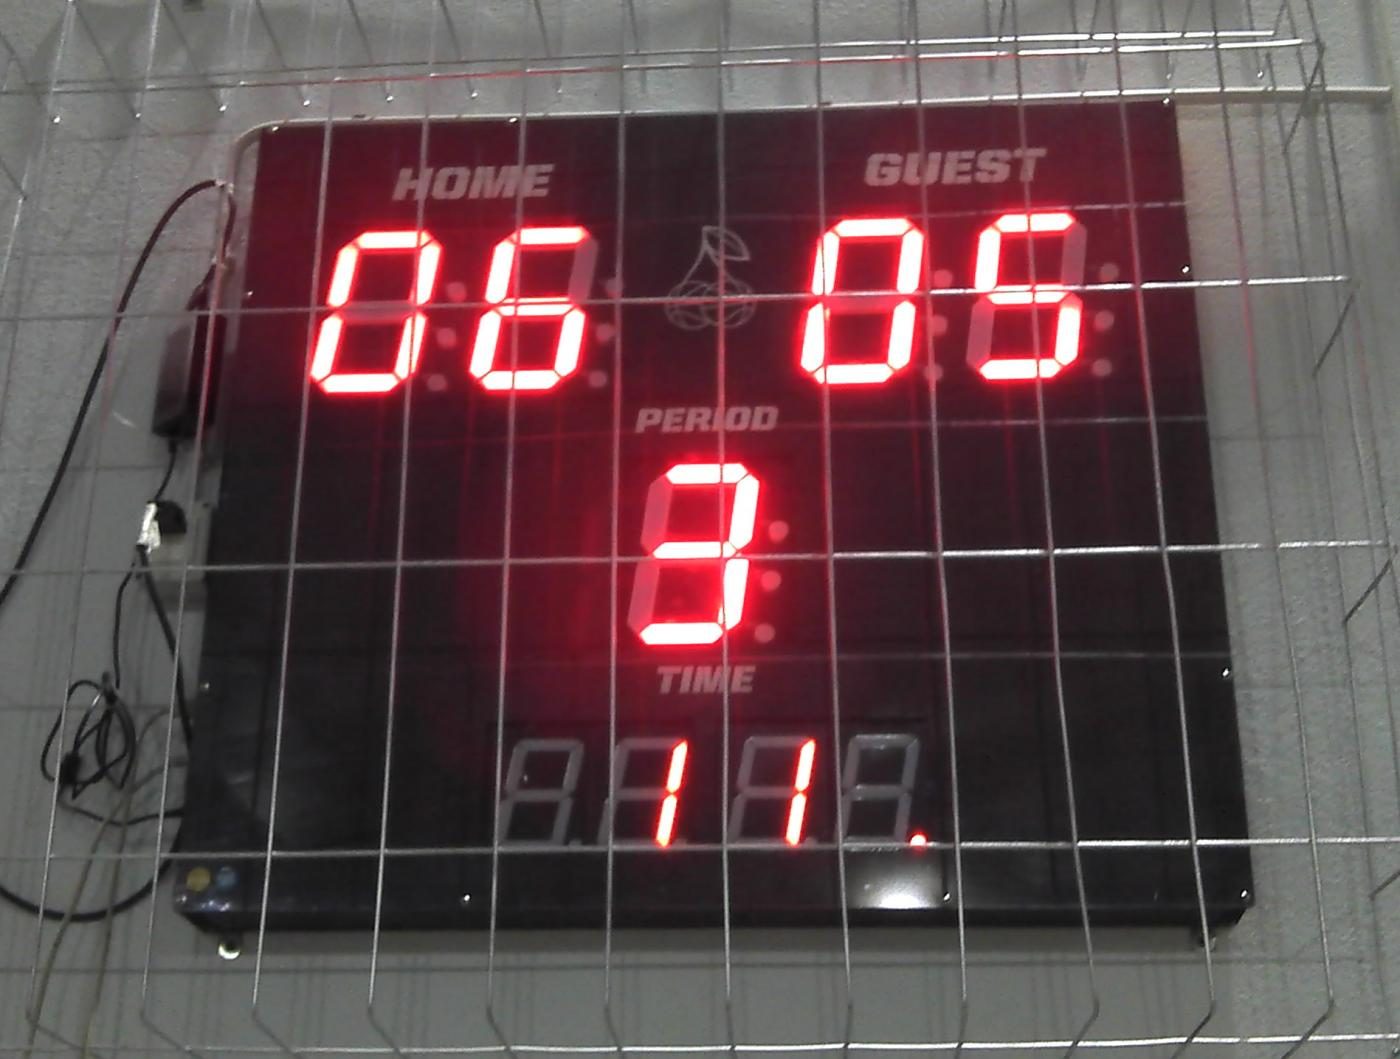
\includegraphics[scale=0.32]{img/Scoreboard_volley}

\caption{ScoreBoard in volleyball mode \label{fig:volleyball-mode}}

\end{figure}

Figure \ref{fig:volleyball-mode} shows the new configuration: the two upper display groups show the score for each team.
The central one shows the current set in the match, and the two at the bottom show the sets won by each team.
In listing \ref{lis:volleyMode} is shown the code responsable for the configuration switch: using the DisplayGroup 
library API the main program cleans the displays configuration when the volleyball mode is activated (row 5) and 
inserts the new configuration (rows 7-16). The same procedure is carried out when the same button is pressed again,
switching back the configuration to basketball mode.

%
\begin{lstlisting}[label=lis:volleyMode,caption=Volleyball mode activation and deactivation]
volleyMode = !volleyMode;

if (volleyMode) {
  // Volleyball mode
  disManager.clearGroups();

  disManager.addGroup(0, 2, &vScore.home, gDigits7, sizeof(gDigits7));
  disManager.addGroup(1, 2, &vScore.away, gDigits7, sizeof(gDigits7));
  disManager.addGroup(2, 1, &vSets.actSet, gDigits7, sizeof(gDigits7));
  disManager.addGroup(3, 1, NULL);
  disManager.addGroup(4, 1, &vSets.homeSet, gDigits4, sizeof(gDigits4));
  disManager.addGroup(5, 1, &vSets.awaySet, gDigits4, sizeof(gDigits4));
  disManager.addGroup(6, 1, NULL);

  disManager.enableGroup(3, false);
  disManager.enableGroup(6, false);

} else {
  // Basketball mode
  disManager.clearGroups();
  
  disManager.addGroup(0, 2, &bScore.home, gDigits7, sizeof(gDigits7));
  disManager.addGroup(1, 2, &bScore.away, gDigits7, sizeof(gDigits7));
  disManager.addGroup(2, 1, &time.period, gDigits7, sizeof(gDigits7));
  disManager.addGroup(3, 2, &time.min, gDigits4, sizeof(gDigits4));
  disManager.addGroup(4, 2, &time.sec, gDigits4, sizeof(gDigits4));
}
\end{lstlisting}

The input mode must be setupMode and one button will allow the user to switch between basketball mode and 
volleyball mode. Two groups are disabled (rows 15-16) because they are not used to show the number of 
sets won by the two teams (a digit is enough for each team!).
The switch can be carried out on the fly, at runtime, and all the information regarding on mode or the other 
are kept back in the respective variables; thus when the user switches back to one mode he will find the displays 
in the same state they were when he left that mode. This works only if there hasn't been any power cycle in between, 
because the backup on the EEPROM memory works only for basketball mode. 

\end{document}



